\newcommand{\lecturetitle}[1]{
  \title{01204211 Discrete Mathematics \\ #1}
  \author{Jittat Fakcharoenphol}
  \frame{\titlepage}
}

\lecturetitle{Lecture 9: Counting 1}

\begin{frame}\frametitle{Let's count}
  \begin{tcolorbox}
    {\bf Club representatives:} You are a second year student. Your
    board game club has 40 members which are in the first year.  There
    is a big competition very soon, so the club has to find exactly 2
    representatives (from the first-year students) for the competition.
  \end{tcolorbox}
  \pause

  \begin{itemize}
  \item
    How to find these 2 representatives?  One of your friends suggests
    that to be fair to everyone, you have to look at every possible
    pair and see how the 2 members of the pair play together as a
    team.  \pause
  \item
    It might take a very long time, you think.  How many pairs are
    there?
  \end{itemize}
\end{frame}

\begin{frame}\frametitle{Club representatives (1)}
  \begin{itemize}
  \item
    To choose the member of the pair, you pick the first member and then
    pick the second member.  \pause
  \item There are 40 ways to choose the
    first member. \pause For every person you pick as the first member,
    there are exactly 39 left to pick as the second one. \pause
    Therefore, there are $40\cdot 39 = 1,560$ ways.  \pause
  \item
    Wait.. \pause This is over counting.  Picking $a$ as the first
    member and $b$ as the second member results in the same pair as
    picking $b$ first and $a$ second. \pause Thus, every pair is counted
    twice.  \pause
  \item The correct number of pairs is 780; too many possibilities to
    consider, you conclude.
  \end{itemize}
\end{frame}

\begin{frame}\frametitle{Club representatives (2)}
  \begin{itemize}
  \item Since 780 is too many, you decide to randomly choose 15 pairs
    of representatives and observe how each pair plays.
    \pause
  \item Your friend argue that 15 is too small.  Because the number of
    members is 40 and we will miss someone there.
    \pause
  \item So you ask, how many pairs one have to randomly choosing a
    pair from 40 members so that it is very likely that every member
    is picked once?
    \pause
  \item You try to calculate the number, but your friend starts
    writing a program to simulate.
  \end{itemize}
\end{frame}

\begin{frame}\frametitle{Club representatives (2)}
  \begin{itemize}
  \item Here's the table of the simulation.  For each value of number
    of random pairs, 2,000 simulations has been conducted.

    \vspace{0.1in}
    
    {\small
    \begin{tabular}{c|c}
      \hline
      Number of pairs to random & \% of choosing everyone once \\
      \hline
      20 & 0.00 \\
      30 & 0.00 \\
      40 & 0.15 \\
      50 & 2.45 \\
      60 & 12.05 \\
      80 & 51.65 \\
      100 & 78.00 \\
      120 & 91.25 \\
      140 & 97.10 \\ \hline
    \end{tabular}
    }
    \pause

  \item You end up choosing randomly 100 pairs, as it has about 80\%
    chance.  You feel so tired, but you keep wondering if you can
    calculate the number without having to write a program.
  \end{itemize}
\end{frame}

\begin{frame}\frametitle{Club representative again (1)}
  \begin{tcolorbox}
    {\bf A team:} Another team competition is coming up.  It requires
    a team of 5 players.  In the team, each player can play either as
    Protoss, Terrans, or Zerg.  Luckily, only one team of 5 members
    volunteers to participate.
  \end{tcolorbox}

  \begin{itemize}
  \item
    To find the best team organization, you ask them to try all
    possible configurations of race choices against AI players.  How
    many games do you have to watch?  \pause
  \item
    Each member has 3 choices and this member's choice is independent
    of the other.  Therefore, there are $3\cdot 3\cdot 3\cdot 3\cdot 3
    = 243$ possible ways. \pause
  \item
    You are still tired from watching 100 pairs of players.  So you
    change your mind and ask them to try only configurations that
    contain all the three races.  How many are there?
  \end{itemize}
\end{frame}

\begin{frame}\frametitle{Club representative again (2)}
  \begin{itemize}
  \item Your old friend asks you if you need a computer program.  You
    say 'No', and try to think of the answer.
    \pause
  \item You come up with an idea.  Instead of counting ``good
    configurations'', let's count ``bad'' ones, i.e., configurations
    that miss some race.
    \pause
    \begin{itemize}
    \item Configurations containing one race: $3$
      \pause
    \item Configurations containing only two races, say, Protoss and
      Terrans: each person has 2 choices; therefore, there are $2\cdot
      2\cdot 2\cdot 2\cdot 2 = 32$ configurations.
      \pause
    \item There are 3 ways to have two races.  Therefore, there are
      $32\cdot 3 = 96$ ways.
      \pause
    \item Thus, the number of good configurations is $243 - 96 - 3 =
      144$ ways.
    \end{itemize}
    \pause
  \item That's not too many.  So you let them play 144 games.  \pause
    It turns out that 144 is wrong.
  \item Can you spot the mistake?
  \end{itemize}
\end{frame}

\begin{frame}\frametitle{Club representative again (3)}
  \begin{itemize}
  \item Again, we over-count some configuration,  \pause e.g., the
    configuration where all players play Protoss is counted 3 times.
    \pause
  \item In fact, it appears the first time we count single race
    configurations, appears when we count Protoss-Terrans, and finally
    appears when we count Protoss-Zerg.
    \pause
  \item The number of bad configurations is $96 - 3$. \pause
  \item The correct number of games would be $243 - (96 - 3) = 150$.
  \end{itemize}
\end{frame}

\begin{frame}\frametitle{Sets: quick review (1)}
  \begin{itemize}
  \item Sets are very important notions in mathematics.  A {\bf set}
    is a collection of elements.
  \item Common set of numbers: real numbers ${\mathbb R}$, integers
    ${\mathbb Z}$, rational numbers ${\mathbb Q}$, positive integers
    ${\mathbb N}$.
  \item There are many ways to specify sets.
    \begin{itemize}
    \item By listing all elements: $\{2,3,5,7,11\}$
    \item By describing its elements: $\{ \mbox{all prime numbers} \}$
    \item By filtering elements from other sets: $\{ p\in {\mathbb N} : \mbox{$p$ is a prime}\}$.
    \end{itemize}
  \end{itemize}
\end{frame}

\begin{frame}\frametitle{Sets: quick review (2)}
  \begin{itemize}
  \item If $a$ is an element of $S$, we write $a\in S$.  The {\bf
    cardinality} of a set is the number of its elements.  We denote by
    $|A|$, the cardinality of $A$.
  \item Note that $|\{2,3,5,7,11\}|=5$ and $|{\mathbb Z}|=\infty$.  A
    set whose cardinality is zero is called an {\bf empty set},
    denoted by $\emptyset$.
  \item If every element of $A$ is also an element of $B$, we say that
    $A$ is a {\bf subset} of $B$, denoted by $A\subseteq B$.  For
    example,
    \begin{itemize}
    \item $\{1,3\}\subseteq\{1,2,3,4\}$
    \item ${\mathbb Z}\subseteq{\mathbb Q}\subseteq{\mathbb R}$
    \item $\{ p\in{\mathbb N} : \mbox{$p$ is prime and $p>2$}\}\subseteq\{ x\in{\mathbb N} : \mbox{$x$ is odd}\}$
    \end{itemize}
    Note that $A\subseteq A$ and $\emptyset\subseteq A$.
  \item If $A\subseteq B$ but $A\neq B$, we write $A\subset B$.
  \end{itemize}
\end{frame}

\begin{frame}\frametitle{Set operations}
  Suppose that we are given two sets $A$ and $B$.
  \begin{itemize}
  \item An {\bf intersection}, denoted by $A\cap B$, is a set whose
    elements are elements of both $A$ and $B$.
  \item A {\bf union}, denoted by $A\cup B$, is a set whose elements
    are elements of $A$ or $B$.
  \item A {\bf difference} of $A$ and $B$, denoted by $A\setminus B$
    or $A-B$, is a set whose elements are elements of $A$ but not
    elements of $B$.
  \end{itemize}

  Note that
  \begin{itemize}
  \item $A\cap B\subseteq A$
  \item $A\subseteq A\cup B$
  \item $A\setminus B \subseteq A$
  \item If $A\subseteq B$, then $A\setminus B = \emptyset$.
  \end{itemize}
\end{frame}

\begin{frame}\frametitle{The number of subsets\footnote{Materials on counting mostly follows [LPV].}}
  \begin{itemize}
  \item Let's get back to counting.  Our next question: {\em What is the
    number of all subsets of a set with $n$ elements?}
    \pause
  \item There are many ways to figure out the answer.  Sometimes it is
    useful to start by looking at small examples.
    \pause
  \item Note that the actual set itself does not matter, i.e., the
    numbers of subsets of $\{1,2,3,4\}$ and $\{a,b,c,d\}$ are equal.
    \begin{itemize}
    \item $\emptyset$ has \pause 1 subset: itself.
    \item $\{1\}$ has \pause 2 subsets: $\emptyset$ and $\{1\}$.
    \item $\{1,2\}$ has \pause 4 subsets.
    \item $\{1,2,3\}$ has \pause 8 subsets.
    \end{itemize}
    \pause
  \item We can guess that the answer is $2^n$.  But how can we prove
    that?
  \end{itemize}
\end{frame}

\begin{frame}\frametitle{Choosing a subset (1)}
  \begin{itemize}
  \item Let's try to think about how to select a subset.  To be
    concrete, let's consider choosing a subset of set $\{1,2,3\}$.
  \item There are many ways to do so, but let's follow an obvious one:
    consider each element and make a decision.
    \pause
    \begin{itemize}
    \item 1st step: we have a choice of choosing $1$ or not choosing
      $1$: $2$ choices.
      \pause
    \item 2nd step: let's consider $2$.  Whatever the decision that we
      make on $1$, we have 2 choices for $2$.
      \pause
    \item 3rd step: let's consider $3$. Whatever the decision that we
      make on $1$ and $2$, we again have 2 choices for $3$.
    \end{itemize}
    \pause
  \item This concludes that we have, in total, $2\cdot 2\cdot 2=8$
    ways of choosing subsets of set $\{1,2,3\}$.
  \end{itemize}
\end{frame}

\begin{frame}\frametitle{A decision tree}
  We describe the process as a decision tree for choosing subset $S$
  from $A=\{1,2,3\}$.

  {\tiny
  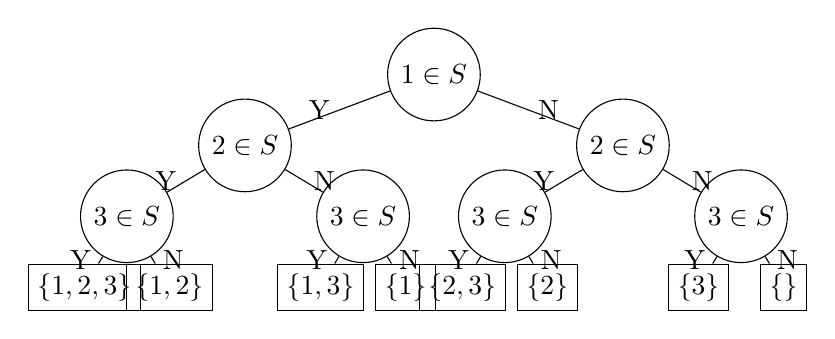
\begin{tikzpicture}[scale=0.6]
    \tikzstyle{level 1}=[sibling distance=80mm] 
    \tikzstyle{level 2}=[sibling distance=50mm] 
    \tikzstyle{level 3}=[sibling distance=18mm] 

    \node [circle, draw] (a){$1\in S$}
      child {node [circle, draw] (b) {$2\in S$}
        child {node [circle, draw] (c) {$3\in S$}
          child {node [rectangle, draw] (d) {$\{1,2,3\}$}}
          child {node [rectangle, draw] (e) {$\{1,2\}$}}
        }
        child {node [circle, draw] (f) {$3\in S$}
          child {node [rectangle, draw] (g) {$\{1,3\}$}}
          child {node [rectangle, draw] (h) {$\{1\}$}}
        }
      }
      child {node [circle, draw] (i) {$2\in S$}
        child {node [circle, draw] (j) {$3\in S$}
          child {node [rectangle, draw] (k) {$\{2,3\}$}}
          child {node [rectangle, draw] (l) {$\{2\}$}}
        }
        child {node [circle, draw] (m) {$3\in S$}
          child {node [rectangle, draw] (n) {$\{3\}$}}
          child {node [rectangle, draw] (o) {$\{\}$}}
        }
      };
    \path (a) -- (b) node [midway, left] {Y};
    \path (a) -- (i) node [midway, right] {N};

    \path (b) -- (c) node [midway, left] {Y};
    \path (b) -- (f) node [midway, right] {N};

    \path (c) -- (d) node [midway, left] {Y};
    \path (c) -- (e) node [midway, right] {N};

    \path (f) -- (g) node [midway, left] {Y};
    \path (f) -- (h) node [midway, right] {N};

    \path (i) -- (j) node [midway, left] {Y};
    \path (i) -- (m) node [midway, right] {N};

    \path (j) -- (k) node [midway, left] {Y};
    \path (j) -- (l) node [midway, right] {N};

    \path (m) -- (n) node [midway, left] {Y};
    \path (m) -- (o) node [midway, right] {N};
  \end{tikzpicture}
  }
\end{frame}

\begin{frame}\frametitle{Choosing a subset (2)}
  \begin{itemize}
  \item To be concrete, let's consider choosing a subset of set
    $\{1,2,3\}$.
  \item We make 3 decisions, for all elements in the set.  The number
    of ways we can choose a subset is 8.
  \item While we know that it is the correct answer, let's look back
    on what we are trying to do. \pause
  \item We are trying to count the number of subsets. \pause But we
    are actually counting the number of ways we can choose a subset.
  \item To make sure that they are the same number, we need to make
    sure that: \pause
    \begin{itemize}
    \item We count everything: for every possible subset, there is at
      least one way we can choose it.
    \item We do not over count: any two different ways of choosing
      subsets produce two different subsets.
    \end{itemize}
  \end{itemize}
\end{frame}

\begin{frame}\frametitle{The number of subsets}
  Let's think about a general case for set $A=\{1,2,\ldots,n\}$ with
  $n$ elements.  \pause We choose elements of a subset in $n$ steps.
  Each step $i$, for $1\leq i\leq n$, we consider $i\in A$, and we
  have $2$ choices.  \pause Hence, there are $2^n$ ways of choosing
  subsets.
  {\small
    \begin{itemize}
    \item {\bf To see that we can choose every subset:} \pause
      consider a given subset $S\subseteq A$.  Note that we when we
      consider $i$, we can choose $i$ if and only if $i\in S$.  \pause
    \item {\bf To see that two different ways of choosing subsets
      produce different subsets:} \pause consider two different ways
      of choosing subsets.  Since they differ in some step, let $i\in
      A$ be the element that they choose differently.  Thus, one of
      the subsets contain $i$ while the other does not.
    \end{itemize}
  }
  \pause

  Therefore, we have proved the following theorem.

  \begin{tcolorbox}
    {\bf \textcolor{blue}{Theorem:}} The number of subsets of a set with
    $n$ elements is $2^n$.
  \end{tcolorbox}
\end{frame}
